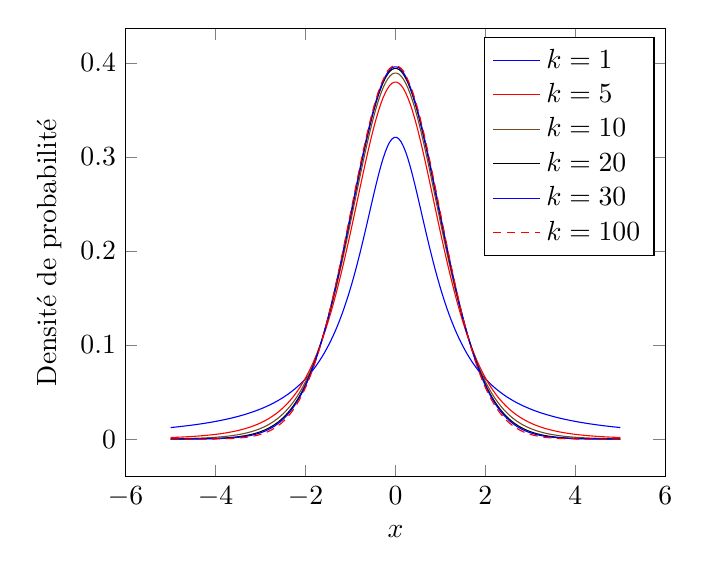
\begin{tikzpicture}[
    declare function={
      gamma(\z)=(2.506628274631*sqrt(1/\z)+ 0.20888568*(1/\z)^(1.5)+ 0.00870357*(1/\z)^(2.5)- (174.2106599*(1/\z)^(3.5))/25920- (715.6423511*(1/\z)^(4.5))/1244160)*exp((-ln(1/\z)-1)*\z);},
    declare function={
      student(\x,\k) = (1/sqrt(3.14159265359*\k))*gamma((\k+1)/2)/gamma(\k/2)*(1+\x*\x/\k)^(-(\k+1)/2);}
]
\begin{axis}[
  xlabel = $x$,
  ylabel = {Densité de probabilité},
  samples = 200,
  restrict y to domain = 0:0.5,
  domain = -5:5,
  legend cell align=left]
    \foreach \k in {1, 5, 10, 20, 30, 100} {
      \addplot+[mark={}] {student(x,\k)}; \addlegendentryexpanded{$k=\k$}}
  \end{axis}
\end{tikzpicture}
